%% ID: braking_a_car
%% TITLE: Braking a Car
%% TYPE: question
%% QUESTIONTYPE: numeric
%% CONCEPTS: energy, eq_of_motion_diff, resolving_vectors
%% VIDEOS: 
%% LEVEL: 4
%% TOPIC: mechanics/dynamics
%% ORDER: 6

\begin{problem}[A1961AMIQ2a] %Not too difficult question that relies mainly on knowing Power = Force * velocity and F=ma
{\begin{enumerate}
	\item \question[a]{When a car of mass \quantity{1000}{kg} is travelling along a level road at a steady \quantity{20}{m\,s\sup{-1}}, its engine is working at \quantity{18}{kW}. Find the total resistance due to friction, which may be taken to be constant.}
	\item \question[b]{The engine is suddenly disconnected and the brakes applied, and the car comes to rest in \quantity{50}{m}. Find the force, assumed constant, exerted by the brakes.}
	\item \question[c]{Find also the distance in which the car would come to rest if the engine were disconnected and the brakes applied on an upward incline of angle \vari{\theta}, where \valuedef{\sin(\theta)}{\frac{1}{20}}{}}.
	\item \question[d]{By how much does this change if the car is travelling down the same hill?
\end{enumerate}
}
{
\stress{Adapted with permission from UCLES, A Level Applied Mathematics, June~1961, Paper~1, Question~2.}
}
\answer[a]{Sketching a diagram of the forces on the car, as in Figure \ref{fig:Dynamics_car_forces}, is a key first step. The formula relating force, power and velocity at constant velocity is \vari{P} $=$ \valuedef{\vtr{F}\cdot\vtr{v}}{Tv}{} where \vari{P} is the power, \vari{T} the magnitude of the thrust (the forward force \vari{\vtr{F}}) in the direction of the velocity and \vari{v} the speed. This formula is a vector formula, and so \vari{\vtr{F}} and \vari{\vtr{v}} must be in the same direction to simplify it. Since the car is moving at a constant \quantity{20}{m\,s\sup{-1}} (i.e. no acceleration), the forces on the car must balance and so the forward thrust, \vari{T}, must equal the resistive force, \vari{F_{r}}; \valuedef{T}{F_{r}}{}.

\begin{figure}[h]
\centering
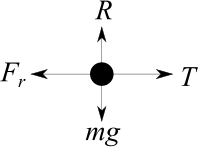
\includegraphics[width=0.2\textwidth]{../../../figures/Dynamics_car_forces.svg}
\caption{} \label{fig:Dynamics_car_forces}
\end{figure}
Rearranging the formula for power and substituting in \vari{F_{r}} gives \vari{T} $=$ \valuedef{\frac{P}{v}}{F_{r}}{} and thus that the total resistance due to friction \vari{F_{r}} $=$ \valuedef{\frac{18000}{20}}{900}{N}.

\answer[b]{ To find the force from the brakes, \vari{F_{b}}, it is easiest to first find the deceleration of the car and then use Newton's Second Law to find the force. Since the force is constant, the acceleration is constant and so the SUVAT equations can be used. We need an equation that does not include \vari{t}, so \valuedef{v^{2}}{u^{2} + 2as}{} is the SUVAT equation to rearrange. The magnitude of the acceleration is then
\begin{equation*}
  a = \frac{v^{2} - u^{2}}{2s} = \frac{(0)^{2} - (20)^{2}}{2 \: (50)} = \mbox{\quantity{-4}{m\,s\sup{-1}}} 
  \end{equation*}
where the negative value reflects the fact that this is actually a deceleration: the car is slowing to a stop. Using \valuedef{\vtr{F}}{m\vtr{a}}{} we find that the total decelerating force is \vari{F} $=$ \valuedef{(1000) \times (4)}{4000}{N} where the minus sign has been dropped on the understanding this force acts against the forward motion. The total decelerating force \valuedef{F}{F_{r} + F_{b}}{} and so \valuedef{F_{b}}{3100}{N}.}
\answer[c]{Again we can assume that the decelerating force is constant, but this time we want to find the distance and we know the force. Consider the forces acting on the car; now the weight has a component in the direction of deceleration and so this must be taken into account. Drawing a diagram of the forces and exaggerating the angle, as in Figure \ref{fig:Dynamics_car_slope_forces}, makes seeing this much easier.
\begin{figure}[h]
\centering
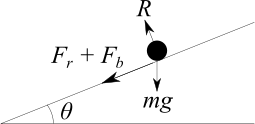
\includegraphics[width=0.3\textwidth]{../../../figures/Dynamics_car_slope_forces.svg}
\caption{} \label{fig:Dynamics_car_slope_forces}
\end{figure}


The total decelerating force is thus the sum of all forces acting down the plane of the slope: \valuedef{F}{F_{r} + F_{b} + mg \sin(\theta)}{}. To solve this problem we only ever need \vari{\sin(\theta)} and not \vari{\theta] itself, and so the information in the question can be used directly. An alternate way of stating that \valuedef{\sin(\theta)}{\frac{1}{20}}{} is \valuedef{\theta}{\arcsin(\frac{1}{20})}{} or \valuedef{\theta}{\sin^{-1}(\frac{1}{20})}{} and this is used commonly to avoid the need for using a calculator.
\begin{equation*} 
a = \frac{F}{m} = \frac{- (F_{b} + F_{r} + mg\sin(\theta) )}{m} = \frac{- ((3100) + (900) + (490))}{(1000)} = \mbox{\quantity{-4.49}{m\,s\sup{-2}}}
\end{equation*}
The SUVAT equation can now be used to find the distance it takes the car to come to rest:
\begin{equation*} 
s = \frac{v^{2} - u^{2}}{2a} = \frac{(0)^{2} - (20)^{2}}{2 \: (-4.49)} = \mbox{\quantity{44.5}{m}} 
\end{equation*}}

	\answer[d]{The last part of the question is a simple alteration to the previous part; all that is required is to realise that gravity now acts against the decelerating forces and so now the acceleration is:
\begin{equation*} 
 a = \frac{F}{m} = \frac{- (F_{b} + F_{r} - mg\sin(\theta) )}{m} = \frac{- ((3100) + (900) - (490))}{(1000)} = \mbox{\quantity{-3.51}{m\,s\sup{-2}}}
\end{equation*}
and so the stopping distance increases to:
\begin{equation*} 
s = \frac{v^{2} - u^{2}}{2a} = \frac{v^{2} - u^{2}}{2 \frac{F}{m}} = \frac{(0)^{2} - (20)^{2}}{2 \: (-3.51)}
= \mbox{\quantity{57.0}{m}}
 \end{equation*}
which is nearly a \quantity{13}{m} difference in braking distance on a \quantity{5}{\%} gradient, depending on direction of travel.

}
\end{problem}